\documentclass{article}\usepackage[]{graphicx}\usepackage[]{color}
%% maxwidth is the original width if it is less than linewidth
%% otherwise use linewidth (to make sure the graphics do not exceed the margin)
\makeatletter
\def\maxwidth{ %
  \ifdim\Gin@nat@width>\linewidth
    \linewidth
  \else
    \Gin@nat@width
  \fi
}
\makeatother

\definecolor{fgcolor}{rgb}{0.345, 0.345, 0.345}
\newcommand{\hlnum}[1]{\textcolor[rgb]{0.686,0.059,0.569}{#1}}%
\newcommand{\hlstr}[1]{\textcolor[rgb]{0.192,0.494,0.8}{#1}}%
\newcommand{\hlcom}[1]{\textcolor[rgb]{0.678,0.584,0.686}{\textit{#1}}}%
\newcommand{\hlopt}[1]{\textcolor[rgb]{0,0,0}{#1}}%
\newcommand{\hlstd}[1]{\textcolor[rgb]{0.345,0.345,0.345}{#1}}%
\newcommand{\hlkwa}[1]{\textcolor[rgb]{0.161,0.373,0.58}{\textbf{#1}}}%
\newcommand{\hlkwb}[1]{\textcolor[rgb]{0.69,0.353,0.396}{#1}}%
\newcommand{\hlkwc}[1]{\textcolor[rgb]{0.333,0.667,0.333}{#1}}%
\newcommand{\hlkwd}[1]{\textcolor[rgb]{0.737,0.353,0.396}{\textbf{#1}}}%

\usepackage{framed}
\makeatletter
\newenvironment{kframe}{%
 \def\at@end@of@kframe{}%
 \ifinner\ifhmode%
  \def\at@end@of@kframe{\end{minipage}}%
  \begin{minipage}{\columnwidth}%
 \fi\fi%
 \def\FrameCommand##1{\hskip\@totalleftmargin \hskip-\fboxsep
 \colorbox{shadecolor}{##1}\hskip-\fboxsep
     % There is no \\@totalrightmargin, so:
     \hskip-\linewidth \hskip-\@totalleftmargin \hskip\columnwidth}%
 \MakeFramed {\advance\hsize-\width
   \@totalleftmargin\z@ \linewidth\hsize
   \@setminipage}}%
 {\par\unskip\endMakeFramed%
 \at@end@of@kframe}
\makeatother

\definecolor{shadecolor}{rgb}{.97, .97, .97}
\definecolor{messagecolor}{rgb}{0, 0, 0}
\definecolor{warningcolor}{rgb}{1, 0, 1}
\definecolor{errorcolor}{rgb}{1, 0, 0}
\newenvironment{knitrout}{}{} % an empty environment to be redefined in TeX

\usepackage{alltt}
%%%%%%%%%%%%%%%%%%%%%%%%%%%%%%%%%%%%%%%%%%%%%%%%%%%%%%%%%%%%%%%%%%%%%%%%%%%%%%%%
% Preample
%%%%%%%%%%%%%%%%%%%%%%%%%%%%%%%%%%%%%%%%%%%%%%%%%%%%%%%%%%%%%%%%%%%%%%%%%%%%%%%%

\usepackage{amsmath}  % Enables the align enviroment
\usepackage{amssymb}  % Math symbols (e.g. \mathbb{})
\usepackage{dsfont} 	% For \mathds{1} blackboard bold 1
\usepackage[footnote,draft,nomargin]{fixme}    % For fixme notes and corrections
\usepackage{hyperref} % For urls and hyperlinks

% For bibliography
\usepackage[numbers]{natbib}

% For colors
\usepackage{color}

% For algorihmns
\usepackage{algorithm}
\usepackage[noend]{algpseudocode}
\makeatletter
\def\BState{\State\hskip-\ALG@thistlm}
\makeatother

% For theorem/props/lemmas
\usepackage{amsthm}
\theoremstyle{plain}
\newtheorem{proposition}{Proposition}
\newtheorem{lemma}{Lemma}

\renewcommand{\algorithmicrequire}{\textbf{Input:}}
\renewcommand{\algorithmicensure}{\textbf{Output:}}


%%%%%%%%%%%%%%%%%%%%%%%%%%%%%%%%%%%%%%%%%%%%%%%%%%%%%%%%%%%%%%%%%%%%%%%%%%%%%%%%
% My math macros
%%%%%%%%%%%%%%%%%%%%%%%%%%%%%%%%%%%%%%%%%%%%%%%%%%%%%%%%%%%%%%%%%%%%%%%%%%%%%%%%

\DeclareMathOperator{\sgn}{sgn}
\DeclareMathOperator*{\maximize}{maximize}
\DeclareMathOperator*{\minimize}{minimize}
\DeclareMathOperator*{\argmax}{arg\,max}
\DeclareMathOperator*{\tr}{tr}
\DeclareMathOperator*{\rank}{rank}
\DeclareMathOperator{\vect}{vec}
\DeclareMathOperator{\arctanh}{arctanh}
\renewcommand{\vec}{\boldsymbol}
\newcommand{\slfrac}[2]{\left.#1\middle/#2\right.}
\newcommand{\panel}[1]{\textsf{#1}}
\newcommand{\bbE}{\mathbb{E}}
\newcommand{\bbR}{\mathbb{R}}
\newcommand{\bbN}{\mathbb{N}}
\newcommand{\calN}{\mathcal{N}}
\newcommand{\calW}{\mathcal{W}}
\newcommand{\bbOne}{\mathds{1}}
\newcommand{\var}{\text{var}}
\newcommand{\mfJ}{\mathfrak{J}}

% Common bold symbols
\newcommand{\vSigma}{{\vec{\Sigma}}}
\newcommand{\hvSigma}{{\hat{\vec{\Sigma}}}}
\newcommand{\vPsi}{{\vec{\Psi}}}
\newcommand{\vDelta}{{\vec{\Delta}}}
\newcommand{\vTheta}{{\vec{\Theta}}}
\newcommand{\hvTheta}{{\hat{\vec{\Theta}}}}
\newcommand{\hvPsi}{{\hat{\vec{\Psi}}}}
\newcommand{\vX}{{\vec{X}}}
\newcommand{\vx}{{\vec{x}}}
\newcommand{\vY}{{\vec{Y}}}
\newcommand{\vS}{{\vec{S}}}
\newcommand{\vU}{{\vec{U}}}
\newcommand{\vD}{{\vec{D}}}
\newcommand{\vI}{{\vec{I}}}
\newcommand{\vJ}{{\vec{J}}}
\newcommand{\vE}{{\vec{E}}}

\newcommand{\fig}[3]{
\begin{figure}
  \begin{center}
    \includegraphics[width=#2]{#1}
  \end{center}
  \vspace{-5mm}
  \caption{\emph{#3}}
  \label{#1}
\end{figure}
}


\title{Graphical meta analysis: Estimation of covariance matrices from multiple studies}
\author{
  Anders Ellern Bilgrau \\ \texttt{abilgrau@math.aau.dk} \and
  Poul Svante Eriksen \\ \texttt{svante@math.aau.dk} \and
  Martin B\o{}gsted \\ \texttt{m\textunderscore{}boegsted@dcm.aau.dk}
}
\IfFileExists{upquote.sty}{\usepackage{upquote}}{}
\begin{document}




\maketitle
\begin{abstract}
This paper proposes a model and estimators for a common covariance matrix in cases where multiple datasets are present and thus provide a basis for meta analysis of gaussian graphical models. Our approach is inspired by traditional meta analysis using random effects models. We derive the basic properties and estimators of the model and compare our estimators method to the straight-forward approaches of simple averages or ``mega analysis'' were the datasets are combined, reprocessed, and plugged into the usual estimators. Though only a modest improvement, explicitly accounting for the inter-study variance is superior to the alternative. The model is also shown to be applicable as an intermediate between linear discriminant analysis (LDA) and quadratic discriminant analysis (QDA). \medskip

\noindent \textbf{Keywords:} \textit{meta analysis, covariance estimation, integrative analysis, network integration, structural meta analysis, gaussian graphical modeling, linear discriminant analysis, quadratic discriminant analysis}
\end{abstract}

\newpage
\tableofcontents


\newpage
\section{Introduction}
The fundamental problem in statistics of accurately and precisely estimating the covariance matrix (or its inverse) is notoriously difficult though computationally easy. The usual bias-corrected maximum likelihood estimator (MLE), the sample covariance matrix, have long been known to perform poorly in general due to high variability \citep{Dempster1972}. The sample covariance is ill-conditioned when the sample size $n$ is less than the number of variables $p$. Because of its central statistical role the list of statistical methods and applications utilizing the estimated covariance matrix is extraordinarily long. Beside the many standard statistical methods such as principal component analysis (PCA), linear discriminant analysis (LDA), quadratic discriminant analysis (QDA), more direct applications include [examples in medicine, biology. genetics, finance, forensics, physics, engineering, signal processing]. Among this expanding list of applications is also an increasing number of high-dimensional applications and datasets publicly available at online repositories.

In high-dimensional datasets the number of features $p$ far exceed the number of samples $n$. Since the number of parameters increase quadratically in $p$ and the sample covariance become singular when $p > n$ a plethora of shrinkage and regularization estimators have been proposed to combat the accompanying problems by effectively increasing the degrees of freedom. Instead of attempting to derive still more sophisticated estimators with diminishing improvements we attempt to alleviate the problem from a different angle by effectively increasing $n$ and using more available data.

We are motivated by gene-gene interaction networks in diffuse large B-cell lymphoma (DLBCL) where the covariance matrix contain all information about the conditional dependencies of the genes. As with many other cancers, a large number of DLBCL studies are now available online and hence we wish to use these studies in combination with our own data to arrive at a good estimate of the covariance matrix and the inter-study variation.




\section{A graphical random effects model}
In a vein similar to regular effect-based meta analysis of \citet{Choi2003}, we think of the the different studies as related but perturbed experiments. The graphical analog to \citet{Choi2003} is the following relatively simple graphical random effects model (GREM) of the observations.
Let $p$ be the number of features and $k$ the number of studies. We model the each sample for the $i$th study as a $p$-dimensional zero-mean multivariate gaussian vector with the covariance matrix realized from a inverse Wishart distribution, i.e.\ the hierarchical model,
\begin{align}
\begin{split} \label{eq:REM}
  \vSigma_i | \vPsi, \nu  &\sim \calW^{-1}(\vPsi, \nu), \\
  \vec{x} | \vSigma_i &\sim \calN_p(\vec{0}_p, \vSigma_i), \qquad i = 1, ..., k,
\end{split}
\end{align}
where $\calW^{-1}(\vPsi, \nu)$ denotes an inverse Wishart distribution with probability density function (pdf),
\begin{align*}
  f(\vSigma_i | \vPsi, \nu) =
  \frac{ |\vPsi|^\frac{\nu}{2} }{
        2^\frac{\nu p}{2} \Gamma_p\!\left( \frac{\nu}{2} \right) }
        |\vSigma_i|^{-\frac{\nu+p+1}{2}}
  e^{-\frac{1}{2} \tr(\vPsi\vSigma_i^{-1})},
\end{align*}
$\vPsi$ and $\vSigma_i$ are positive semi-definite, $\nu > p - 1$, and $\calN_p(\vec{0}_p, \vSigma_i)$ is a multivariate gaussian distribution with pdf
\begin{align*}
f(\vec{x} | \vSigma_i) =
  (2\pi)^{-\frac{p}{2}} \det(\vSigma_i)^{-\frac{1}{2}}
  e^{ -\frac{1}{2}\vec{x}^\top \vSigma_i^{-1}\vx }.
\end{align*}
Throughout this paper, we use generic notation $f(\cdot | \cdot)$ and $f(\cdot)$ for the conditional and unconditional pdf of random variables.
In the model, $\nu$ encodes the inter-study variation where the $\vSigma_i$'s concentrate around $\vPsi$ for $\nu\to\infty$. I.e.\ the inter-study variation goes to zero for larger $\nu$. We wish to infer the parameters $\vPsi$ and $\nu$ from the observed data.




\subsection{The likelihood function}
Suppose we have $n_i$ i.i.d.\ observations, $\vx_{i1}, \dots,\vx_{in_i}$, from the $i = 1,...,k$ independent studies from the model given in \eqref{eq:REM}.
Let $\vX_i = (\vx_{i1}, \dots,\vx_{in_i})^\top$ be the $n_i \times p$ (transposed) expression matrix of the $i$'th study where rows correspond to samples and columns to variables. By the independence assumptions, the log-likelihood is given by
\begin{align*}
  &\ell\!\left(\vPsi, \nu \big|\vX_1, ..., \vX_k  \right)
  = \log f\!\left(\vX_1, ..., \vX_k \big| \vPsi, \nu \right) \\
  &= \log\!\int %\cdots \int
               f(\vX_1, ...,\vX_k |
               \vSigma_1, ..., \vSigma_k, \vPsi, \nu)
             f(\vSigma_1, ..., \vSigma_k | \vPsi, \nu)
             d\vSigma_1 \cdots d\vSigma_k \\
  &= \log\!\int %\cdots \int
               \prod_{i=1}^k
               f(\vX_i | \vSigma_i)
               f(\vSigma_i | \vPsi, \nu)
               d\vSigma_1 \cdots d\vSigma_k \\
  &= \sum_{i=1}^k \log\!\int
               f(\vX_i | \vSigma_i)
               f(\vSigma_i | \vPsi, \nu)
               d\vSigma_i.
\end{align*}
Since the inverse Wishart distribution is conjugate to the multivariate gaussian distribution the integral, of which the integrand forms a gaussian-inverse-Wishart distribution, can be evaluated. Hence $\vSigma_i$ can be marginalized out, cf.\  Appendix \ref{sec:marginalization}, and we arrive at the following expression for the log-likelihood,
\small
\begin{align}
  &\ell\!\left(\vPsi, \nu \big| \vX_1, ..., \vX_k \right) %\notag\\
  = \sum_{i=1}^k \log
    \frac{|\vPsi|^\frac{\nu}{2} \Gamma_p\!\left(\frac{\nu+n_i}{2}\right)}
         {2^\frac{n_i p}{2} |\vPsi +\vX_i^\top\vX_i|^\frac{\nu+n_i}{2}
          \Gamma_p\!\left(\frac{\nu}{2}\right)}          \notag\\
  &= c + \sum_{i=1}^k
            \frac{\nu}{2}  \log |\vPsi|
            + \log \Gamma_p\!\left(\frac{\nu + n_i}{2}\right)
            - \frac{\nu + n_i}{2}\log|\vPsi +\vX_i^\top\vX_i|
            - \log \Gamma_p\!\left(\frac{\nu}{2}\right),
    \label{eq:loglik}
\end{align}
\normalsize
where the constant terms are abbreviated by $c$ and $\Gamma_p$ is the multivariate generalization for the gamma function $\Gamma$, which can be seen in equation \eqref{eq:multigamma} of Appendix \ref{sec:multigamma}. As should be expected, the scatter matrix $\vec{S}_i =\vX_i^\top\vX_i$ and $n_i$ are sufficient statistics for each study.

While we are not able to shown general log-concavity of the log-likelihood, we show that it is log-concave in $\nu$ for fixed $\vSigma$, and hence there exists a unique maxima for the marginal $\ell(\nu)$, cf.\ Appendix \ref{sec:concaveloglik}.
Reversely, for fixed $\nu$ we can show, that the hessian in any stationary point (where $\frac{\partial\ell}{\partial\vPsi} = 0$) is negative semi-definite and hence a local maxima, cf.\ Appendix \ref{sec:negativedefinite}. This combined with the observation that $\ell(\vPsi) \to -\infty$ whenever an eigenvalue $\lambda_i(\vPsi) \to 0$, we conjecture that any stationary point indeed a global maximum.

In the following, estimation of $\vPsi$ for fixed $\nu$ is considered.

\subsection{Moment estimate}
The moment estimate of $\vPsi$ is readily available. It is clear, by construction that the expectation of a single scatter matrix is
\begin{align*}
  &\bbE[ \vec{S}_i ]
    = \bbE[\vX_i^\top\vX_i ]
    = \bbE\left[\bbE[\vX_i^\top\vX_i | \vSigma_i ]\right]
    = \bbE[n_i \vSigma_i]
    = n_i\bbE[\vSigma_i]
    = n_i\frac{\vPsi}{\nu - p - 1}.
\end{align*}
Thus the estimator
\begin{align}
  \hat{\vPsi}
  = \frac{1}{k} \sum_{i = 1}^k \frac{\nu - p - 1}{n_i}\vX_i^\top\vX_i
  = (\nu - p - 1) \frac{1}{k} \sum_{i = 1}^k \frac{1}{n_i}\vS_i
  \label{eq:moment}
\end{align}
of $\vPsi$ is unbiased. This estimate is a scaled average of the empirical covariance matrices.



\subsection{Maximization of the likelihood}
To find the maximizing parameters we differentiate \eqref{eq:loglik} w.r.t.\ $\vPsi$ and equate to zero while assuming $\nu$ known and constant. Assuming $\vPsi$ unstructured, then $\nabla_{\vec{Z}} \log|\vec{Z}| = \vec{Z}^{-1}$ and
\begin{align}
  \vec{0}
%   =\nabla_\vPsi \ell(\vPsi)
  &= \frac{k\nu}{2} \vPsi^{-1}
    - \sum_{i=1}^k \frac{\nu + n_i}{2}
      (\vPsi + \vec{S}_i)^{-1}
  \label{eq:firstordderivloglik} \\
%   &= \frac{k\nu}{2} \vPsi^{-1}
%     - \sum_{i=1}^k \frac{\nu + n_i}{2}
%       (\vPsi(\vec{I} + \vPsi^{-1}\vec{S}_i))^{-1}
%   \notag \\
  &= \frac{k\nu}{2} \vPsi^{-1}
    - \sum_{i=1}^k \frac{\nu + n_i}{2}
      \left(\vec{I} + \vPsi^{-1}\vec{S}_i\right)^{-1}\vPsi^{-1}.
      \notag
\end{align}
While assuming $\vPsi$ unstructured is not strictly correct it (in this case) leads to a valid equation. The proper 1.\ order derivative can in alternative notation be seen in equation \eqref{eq:dloglik} and can easily be seen to be equivalent to the above.
Equation \eqref{eq:firstordderivloglik} is equivalent to
\begin{align*}
    k\nu \vec{I}
    - \sum_{i=1}^k (\nu + n_i)
      \left(\vec{I} - (-\vPsi^{-1}\vec{S}_i)\right)^{-1}
   = \vec{0}.
\end{align*}
which can be rewritten as
\begin{align*}
    k\nu \vec{I}
    - \sum_{i=1}^k      (\nu + n_i)
      \sum_{l=0}^\infty \left(-\vPsi^{-1}\vec{S}_i\right)^{l}
   = \vec{0}.
\end{align*}
by the Neumann series $\left((\vI + \vec{A})^{-1} = \sum_{l = 0}^\infty \vec{A}^l\right)$ if $\lim_{l \to \infty} (I - \vPsi^{-1}\vec{S}_i)^l = \vec{0}$ for all $i$, i.e.\ the eigenvalues of $\vPsi^{-1}\vec{S}_i$ should be less than $1$.

Thus, we can approximate the solution by using the first order expansion $(l = 1)$ and solve for $\vPsi$
\begin{align*}
  \vec{0}
  &= k\nu\vec{I} - \sum_{i=1}^k (\nu + n_i)(\vec{I} - \vPsi^{-1}\vec{S}_i) \\
  &= k\nu\vec{I}
   - k\nu\vec{I}
   - n_\bullet\vec{I}
   + \vPsi^{-1}\sum_{i=1}^k \nu\vec{S}_i
   + \vPsi^{-1}\sum_{i=1}^k n_i\vec{S}_i \\
  &= - n_\bullet\vec{I}
     + \vPsi^{-1}\sum_{i=1}^k (\nu + n_i) \vec{S}_i
\end{align*}
where $n_\bullet = \sum_{i=1}^k n_i$ is the total number of observations. This implies
\begin{align*}
   \vPsi^{-1}\sum_{i=1}^k (\nu + n_i) \vec{S}_i
    = n_\bullet \vec{I}
\end{align*}
which is equivalent to
\begin{align}
  \hat{\vPsi}
  %=  \sum_{i=1}^k \frac{\nu + n_i}{ n_i} \vec{S}_i
  = \frac{\sum_{i=1}^k (\nu + n_i) \vec{S}_i}{n_\bullet}
  = \frac{\sum_{i=1}^k (\nu + n_i)\vX_i^\top\vX_i}{\sum_{i=1}^k n_i},
  \label{eq:mle}
\end{align}
corresponding to a weighted sum of the scatter matrices.




\subsection{Maximization using the EM algorithm}
We now derive the updating scheme of the expectation-maximization (EM) algorithm for fixed $\nu$.
Suppose $\hvPsi_{(t)}$ is the current estimate of $\vPsi$ and that $\vS_i = \vX_i^\top\vX_i = \sum_{j = 1}^{n_i} \vx_{ij} \vx_{ij}^\top$ is the empirical scatter matrix where $\vX_i = (\vx_{i1}, ..., \vx_{in_i})^\top$.
We now compute the expectation step of the EM-algorithm.

From \eqref{eq:REM} we have that,
\begin{align*}
  \vS_i | \vSigma_i  &\sim \calW_p(\vSigma_i, n_i), \qquad i = 1, ..., k\\
  \vSigma_i          &\sim \calW_p^{-1}(\vPsi, \nu)
\end{align*}
Let $\vDelta_i = \vSigma_i^{-1}$ be the precision matrix (or, concentration matrix) and let $\vTheta = \vPsi^{-1}$, then
\begin{align}
  \vS_i | \vDelta_i
  &\sim \calW_p( \vDelta_i^{-1}, n_i)
  &\Leftrightarrow & &
  f(\vS_i | \vDelta_i)
  &\propto
      |\vDelta_i|^{\frac{1}{2}}
       e^{-\frac{1}{2}\tr(\vDelta_i\vS_i)},
  \label{eq:precisiondensity}
  \\
  \vDelta_i
  &\sim \calW_p(\vTheta, \nu)
  &\Leftrightarrow & &
  f(\vDelta_i)
  &\propto
       |\vTheta|^{-\frac{\nu}{2}}
       e^{-\frac{1}{2}\tr(\vTheta^{-1}\vDelta_i)}.
  \notag
\end{align}
From the conjugacy of the inverse Wishart and the Wishart distribution, we have the posterior distribution for the precision matrix,
\begin{align*}
    \vDelta_i | \vS_i
    &\sim \calW_p\!\left( (\vTheta^{-1} + \vS_i)^{-1}, n_i + \nu\right)
\end{align*}
Hence, the expectation step is given by
\begin{align*}
  \bbE[\vDelta_i |\vS_i] = (n_i + \nu)(\vTheta^{-1} + \vS_i)^{-1}.
\end{align*}
The maximization step, in which the log-likelihood $\ell(\vTheta|\vDelta_1, ..., \vDelta_k)$ is maximized, yields the estimate
\begin{align*}
 \hat{\vTheta} = \frac{1}{k\nu}\sum_{i = 1}^k \vDelta_i,
\end{align*}
which is the mean of the scaled precision matrices $\frac{1}{\nu}\vDelta_i$.
The derivation of this estimate can be seen in Appendix \ref{sec:precisionloglik}.
The above yield the updating scheme
\begin{align}
  \label{eq:em}
  \hvTheta_{(t+1)}
  = \frac{1}{k\nu}\sum_{i = 1}^k
    (n_i + \nu)\left(\big(\hvTheta_{(t)}\big)^{-1} + \vS_i\right)^{-1}
\end{align}
for $\vTheta$. The connection to the maximum likelihood estimate is immediately seen through equation \eqref{eq:firstordderivloglik}.

\subsection{Estimation procedure}
We propose an alternating procedure between estimating $\nu$ and $\vPsi$ while keeping the other fixed.
Given parameters $\hat{\nu}_{(t)}$ and $\hvPsi_{(t)}$ at iteration $t$, we we estimate $\hvPsi_{(t+1)}$ using the fixed $\hat{\nu}_{(t+1)}$. Subsequently, find $\hat{\nu}_{(t+1)}$ by standard one-dimensional numerical optimization procedure keeping $\hvPsi_{(t)}$ fixed.
This coordinate ascent-like approach is repeated until convergence.
More precisely, in pseudo-code, we propose the algorithm seen in Algorithm \ref{alg:grem}.
\begin{algorithm}
\caption{Pseudo-code for the GREM estimation procedure}\label{alg:grem}
\begin{algorithmic}[1]
\Procedure{GREM coordinate ascent}{}
\State \algorithmicrequire{
\State \emph{Sufficient data:} $(\vS_1, n_1), ..., (\vS_k, n_k)$
\State \emph{Initial parameters:} $\hvPsi_{(0)}, \hat{\nu}_{(0)}$
\State \emph{Convergence criterion:} $\varepsilon > 0$
}
\State \algorithmicensure{
\State \emph{Parameters:} $\hvPsi_{(t')}, \hat{\nu}_{(t')}$
}
\State
\State \emph{Initialize}: $l_{(0)} \gets \ell(\hvPsi_{(0)}, \hat{\nu}_{(0)})$
\For {$t = 1, 2, 3, ...$}
  \State $\hvPsi_{(t)} \gets U\!\left(\hvPsi_{(t-1)}, \hat{\nu}_{(t-1)}\right)$
  \State $\nu_{(t)} \gets \argmax_\nu \ell\!\left(\hvPsi_{(t)}, \nu\right)$
  \State $l_{(t)} \gets \ell\!\left(\hvPsi_{(t)}, \hat{\nu}_{(t)}\right)$
    \If {$l_{(t)} - l_{(t-1)} < \varepsilon$}
      \State \Return $\left(\hvPsi_{(t)}, \nu_{(t)}\right)$
    \EndIf
 \EndFor
\EndProcedure
\end{algorithmic}
\end{algorithm}
The update function $U$ in the algorithm is be defined by the derived estimators above. That is, equations \eqref{eq:moment}, \eqref{eq:mle}, and \eqref{eq:em} define $U$ to be the moment, approximate MLE, and EM estimate respectively.

\section{Numerical results}


To assess the model and the stability of the estimation procedure we generated data from \eqref{eq:REM} for $p = 10$ variables in $k = 3$ studies each with an equal number of observations, $n = n_1 = n_2 = n_3$. We chose the parameters $\nu = 15$ and
\begin{align*}
\vPsi =
  \begin{bmatrix}
     1 & 0.5 & 0.5 \\
     0.5 & 1 & 0.5 \\
     0.5 & 0.5 & 1 \\
  \end{bmatrix}.
\end{align*}
The number of observations is each study, $n_i$, was varied range $[5,14]$.

We measure the precision of the estimates values against the expected covariance matrix given by
\begin{align*}
  \vSigma = \bbE[\vSigma_i] = \frac{1}{\nu - p - 1}\vPsi.
\end{align*}
Let $\hvPsi$ and $\hat{\nu}$ be the estimates obtained in the model described and let
\begin{align*}
  \hat{\vSigma}_\text{GREM} = \frac{1}{\hat{\nu} - p - 1}\hvPsi
\end{align*}
be an estimate of $\vSigma$. We benchmark this against the pooled covariance matrix,
\begin{align*}
  \hvSigma_\text{pool}
    = \frac{1}{k} \sum_{i = 1}^k \frac{1}{n_i} S_i,
    %= \frac{1}{k} \sum_{i = 1}^k \hvSigma_i.
\end{align*}
as a simple alternative estimate of $\vSigma$.
We benchmark the two against each other using the following sum of squared errors,
\begin{align*}
  \text{SSE}(\hvSigma) = \sum_{i \leq j} \frac{(\hat{\Sigma}_{ij}- \Sigma_{ij})^2}{\var(\Sigma_{ij})}
\end{align*}
where
\begin{align*}
 \var(\Sigma_{ij}) = n(\Psi_{ij}^2 + \Psi_{ii}\Psi_{jj}).
\end{align*}

For each $n$ from $5$ to $14$, the squared sum of errors for each estimator, $\text{SSE}(\hvSigma_\text{GREM})$, and $\text{SSE}(\hvSigma_\text{pool})$ where computed for $500$ datasets and the average of these values seen in figure \ref{fig:num_exp_plot} as function of $n$.
Unsurprisingly, the model outperforms the simple pool average covariance matrix.

\begin{knitrout}\footnotesize
\definecolor{shadecolor}{rgb}{0.969, 0.969, 0.969}\color{fgcolor}\begin{figure}[ht]

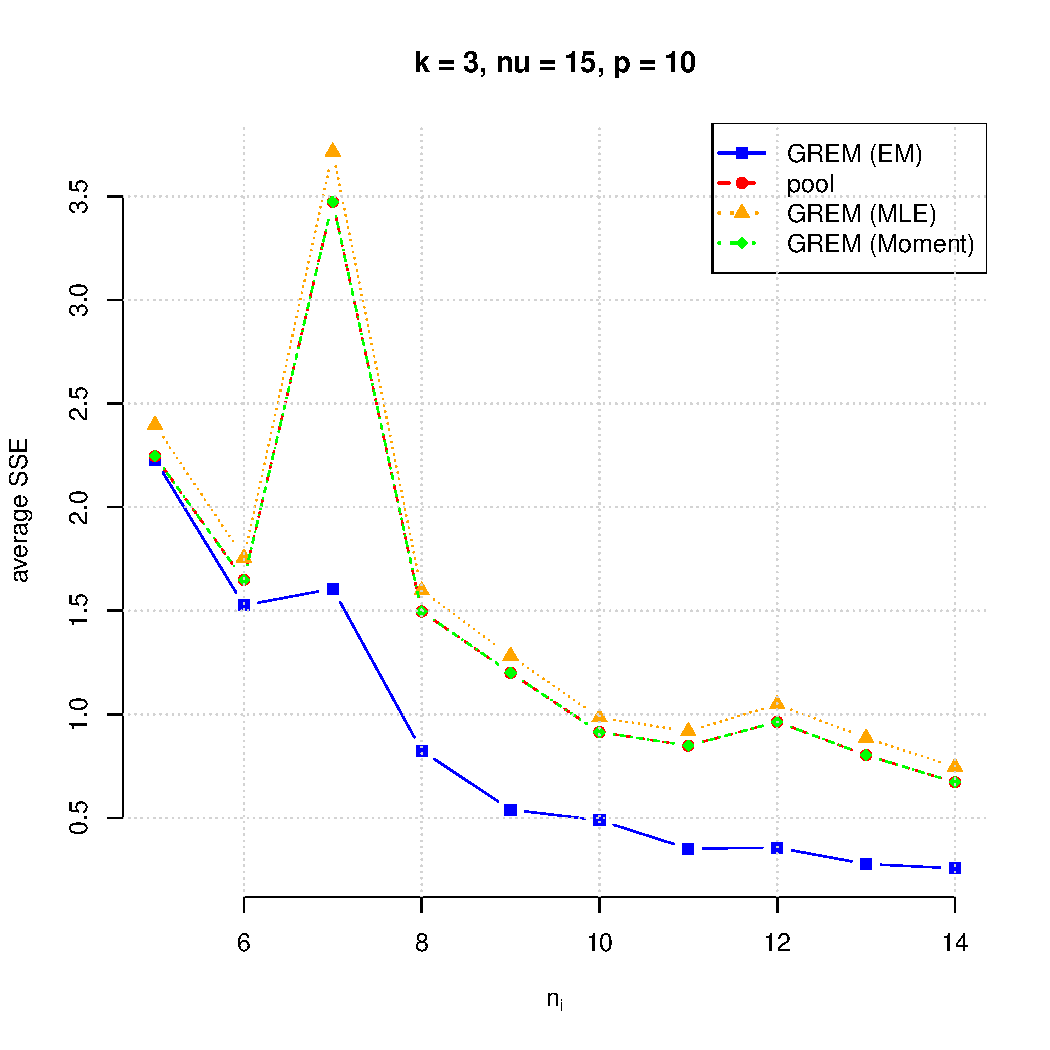
\includegraphics[width=\maxwidth]{figure/num_exp_plot} \caption[]{The average sum or squared errors (SSE), of 500 simulations, as a function of the number of samples $n_i$ in each study.\label{fig:num_exp_plot}}
\end{figure}


\end{knitrout}


\section{Applications}
\subsection{Supervised classification}
The estimate obtained from the model can be utilized in supervised learning as a intermediate case of linear discriminant analysis (LDA) and quadratic discriminant analysis (QDA) to regularized linear discriminant analysis (RDA).

Let $Y$ be a random variable denoting the class $1, ..., k$ and suppose $\vx$ is a random vector of the explanatory variables. Recall, that QDA (and LDA) finds the class $y$ maximizing
\begin{align*}
  P(Y = y | \vX = \vx) =
    \frac{\pi_y f(\vx | Y = y)}
         {\sum_{y' = 1}^k \pi_{y'} f(\vx | Y = y')}
\end{align*}
where $\vx | Y = y$ is assumed multivariate normal, i.e.\
\begin{align*}
  (\vx | Y = y) \sim \calN_p(\vec{\mu}_y, \vSigma_y).
\end{align*}
LDA differs from QDA only by the additional assumption that $\vSigma = \vSigma_y$ for all classes $y$. An intermediate classifier of LDA and QDA can thus be constructed by assuming the $\vSigma_y$'s inversely Wishart distributed as in \eqref{eq:REM}, i.e.\ $\vSigma_y \sim \calW^{-1}(\vPsi, \nu)$. This hierarchical discriminant analysis (HDA) is thus straight-forward to implement given that
\begin{align*}
f(\vx | Y = y)
  &= \int f(\vx| \vSigma_y, Y = y) f(\vSigma_y | Y = y) d\vSigma_y \\
  &= \frac{ |\vPsi|^{\frac{\nu}{2}} \Gamma_p\!\left(\frac{\nu + 1}{2}\right) }
          { \pi^{-\frac{n}{2}} |\vPsi + (\vx-\mu_k)(\vx-\mu_k)^\top|^{\frac{\nu + 1}{2}}
            \Gamma_p\!\left(\frac{\nu}{2}\right)},
\end{align*}
analogous to the computation done in appendix \ref{sec:marginalization}, using the matrix determinant lemma, $|\vec{A} + \vec{u}\vec{v}^\top| = (1 + \vec{v}^\top\vec{A}\vec{u})|\vec{A}|$, to simplify and speed up the computations \citep{}.



\subsection{DLBCL graphical meta analysis}


\section{Concluding remarks}
While the improvements are modest, the results above demonstrate an advantage of modelling the inter-study variance as a hierachical random effects model. However, the virtue of such a model is not from improvement in accuracy alone. Also desireable is the explicit quantification of the inter-study variance. If $\hat{\nu}$ is estimated to be large, the studies exhibit  a largely common covariance structure, and vice-versa when $\hat{\nu}$ is small.

The generalization of the model to $n \gg p$ is extremely interesting though out of scope for this article.



\newpage
\bibliographystyle{plainnat}
\bibliography{references_mendelay,references_manual}


\newpage
\appendix

\section[Marginalization of Sigma]{Marginalization of $\vSigma$}
\label{sec:marginalization}
This sections shows the marginalization out of $\vSigma$ in \eqref{eq:loglik}. For ease of notation we drop the subscript $i$ used in $\vSigma_i$, $\vX_i$, $\vS_i = \vX_i \vX_i^\top$, and $n_i$ in the above text. We do the computation straight-forwardly by the assumptions of the model,
\small
\begin{align*}
  &f(\vX | \vPsi, \nu) \\
  &= \int f(\vX|\vSigma) f(\vSigma | \vPsi, \nu) d\vSigma \\
  &= \int \left[ \prod_{j = 1}^n  (2\pi)^{-\frac{p}{2}} |\vSigma|^{-\frac{1}{2}}
                         e^{-\frac{1}{2}\tr(\vx_i\vx_i^\top\vSigma^{-1})} \right]
          \frac{|\vPsi|^{-\frac{\nu}{2}}}{2^{\frac{\nu p}{2}}\Gamma_p\!\left(\frac{\nu}{2}\right)}
          |\vSigma|^{-\frac{\nu+p+1}{2}}e^{-\frac{1}{2}\tr(\vPsi\vSigma^{-1})}
      \;d\vSigma \\
  &= (2\pi)^{-\frac{np}{2}}
      \frac{|\vPsi|^{-\frac{\nu}{2}}}{2^{\frac{\nu p}{2}}\Gamma_p\!\left(\frac{\nu}{2}\right)}
      \int
        |\vSigma|^{-\frac{n}{2}}  e^{-\frac{1}{2}\tr(\vS\vSigma^{-1})}
        |\vSigma|^{-\frac{\nu+p+1}{2}} e^{-\frac{1}{2}\tr(\vPsi\vSigma^{-1})}
      \;d\vSigma \\
  &=
      \frac{|\vPsi|^{-\frac{\nu}{2}}}{\pi^{-\frac{np}{2}}2^{\frac{(\nu + n) p}{2}}\Gamma_p\!\left(\frac{\nu}{2}\right)}
      \int
        |\vSigma|^{-\frac{(\nu + n)+p+1}{2}}
         e^{-\frac{1}{2}\tr\!\left((\vPsi+ \vS)\vSigma^{-1}\right)}
      \;d\vSigma.
\end{align*}
\normalsize
The integrand here can be recognized as a unnormalized inverse Wishart pdf,  $\calW^{-1}(\vPsi + \vS, \nu + n)$, and so integral evaluates to the reciprocal value of the normalizing constant in that density. Thus,
\begin{align*}
  f(\vX | \vPsi, \nu)
  &=
    \frac{|\vPsi|^{-\frac{\nu}{2}}}
         {\pi^{-\frac{np}{2}} 2^{\frac{(\nu + n) p}{2} } \Gamma_p\!\left(\frac{\nu}{2}\right)}
    \frac{2^\frac{(v+n)p}{2} \Gamma\left(\frac{\nu + n}{2}\right)}
         {|\vPsi + \vS|^{\frac{\nu + n}{2}}} \\
  &=
    \frac{|\vPsi|^\frac{\nu}{2} \Gamma\left(\frac{\nu + n}{2}\right)}
         {\pi^{-\frac{np}{2}} |\vPsi + \vS|^{\frac{\nu + n}{2}}\Gamma_p\!\left(\frac{\nu}{2}\right)},
\end{align*}
which was what was wanted.





\section{Non-concavity of log-likelihood}
\label{sec:concaveloglik}
The log-likelihood is not concave.
This section analyse the (non)-concavity of the log-likelihood function,
\small
\begin{align}
  &\ell\!\left(\vPsi, \nu \big| \vX_1, ..., \vX_k \right) \notag \\
  &= c + \sum_{i=1}^k
            \frac{\nu}{2}  \log |\vPsi|
            + \log \Gamma_p\!\left(\frac{\nu + n_i}{2}\right)  %\notag\\
           - \frac{\nu + n_i}{2}\log|\vPsi +\vS_i|
            - \log \Gamma_p\!\left(\frac{\nu}{2}\right).
            \label{eq:appendloglik}
\end{align}
\normalsize
We first analyze the terms involving $\vPsi$ in \eqref{eq:appendloglik}. Not counting the constant, the first term, $\frac{\nu}{2}  \log | \vPsi |$, is concave by the well known result that the log-determinant of positive semi-definite matrix is concave \citep[See e.g.][pp. 73-74]{Boyd2004}.
The third term in \eqref{eq:appendloglik}, $- \frac{\nu + n_i}{2}\log|\vPsi + \vS_i|$, is convex by the same argument however negated by the sign.
The sum $\vPsi +\vS_i$ is positive semi-definite since both summands are.


Next, we look at the terms involving $\nu$.
Cleary, the mixed terms involving both $\nu$ and $\vPsi$ are log-linear in $\nu$ and hence log-concave.
We thus restrict our attention to the remaining terms not dependent on $\vPsi$.
By themselves, the second term in \eqref{eq:appendloglik},
$
\log \Gamma_p\!\left(\frac{\nu + n_i}{2}\right)
$
is convex since the multivariate gamma function is log-convex, cf.\ section \ref{sec:multigamma}.
In the same manner, the fourth term,
$
  - \log \Gamma_p\!\left(\frac{\nu}{2}\right),
$
is concave by the negative sign.
The sum however of these terms involving $\Gamma_p$ are concave in $\nu$, since
\begin{align*}
  &\log\Gamma_p\!\left( \frac{\nu + n_i}{2} \right) -
    \log\Gamma_p\!\left( \frac{\nu}{2} \right)
  =  \log\frac{\Gamma_p\!\left( \frac{\nu + n_i}{2} \right)}{
                \Gamma_p\!\left( \frac{\nu}{2}       \right)}
  = \log \prod_{j = 1}^p
    \frac{\Gamma\!\left( \frac{\nu + 1 - j}{2} + \frac{n_i}{2} \right)}{
          \Gamma\!\left( \frac{\nu + 1 - j}{2} \right)}.
\end{align*}
which can be seen to be concave since $n_i \geq 2$ for all $i$ and
\begin{align}
  x \mapsto \log\left(\frac{\Gamma(x + a)}{\Gamma(x)}\right)
  \label{eq:logGammaRatio}
\end{align}
is concave for all $x>0$ and $a > 0$. While we do not provide a proof of this the mapping is plotted in figure \ref{fig:log_gamma_ratio}.
Hence, the log-likelihood is log-concave in $\nu$.
\begin{knitrout}\footnotesize
\definecolor{shadecolor}{rgb}{0.969, 0.969, 0.969}\color{fgcolor}\begin{kframe}
\begin{alltt}
\hlstd{logGammaRatio} \hlkwb{<-} \hlkwa{function}\hlstd{(}\hlkwc{x}\hlstd{,} \hlkwc{a}\hlstd{) \{}
  \hlkwd{log}\hlstd{(}\hlkwd{gamma}\hlstd{(x} \hlopt{+} \hlstd{a)}\hlopt{/}\hlkwd{gamma}\hlstd{(x))}
\hlstd{\}}
\hlstd{xs} \hlkwb{<-} \hlkwd{seq}\hlstd{(}\hlnum{0.01}\hlstd{,} \hlnum{2}\hlstd{,} \hlkwc{by} \hlstd{=} \hlnum{0.01}\hlstd{)}
\hlkwd{par}\hlstd{(}\hlkwc{mfrow} \hlstd{=} \hlkwd{c}\hlstd{(}\hlnum{1}\hlstd{,}\hlnum{2}\hlstd{),} \hlkwc{mar} \hlstd{=} \hlkwd{c}\hlstd{(}\hlnum{2}\hlstd{,}\hlnum{2}\hlstd{,}\hlnum{0}\hlstd{,}\hlnum{0}\hlstd{)}\hlopt{+} \hlnum{0.5}\hlstd{)}
\hlkwd{plot}\hlstd{(xs,} \hlkwd{logGammaRatio}\hlstd{(xs,} \hlkwc{a} \hlstd{=} \hlnum{1e-3}\hlstd{),} \hlkwc{type} \hlstd{=} \hlstr{"l"}\hlstd{,} \hlkwc{xlab} \hlstd{=} \hlstr{""}\hlstd{,} \hlkwc{ylab} \hlstd{=} \hlstr{""}\hlstd{)}
\end{alltt}
\end{kframe}\begin{figure}[ht]

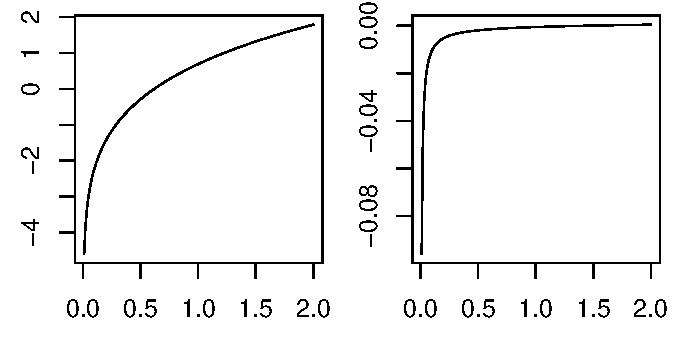
\includegraphics[width=\maxwidth]{figure/log_gamma_ratio} \caption[]{Plots of the mapping given in \eqref{eq:logGammaRatio} for diffent values of $a$.\label{fig:log_gamma_ratio}}
\end{figure}


\end{knitrout}



\subsection{log-convexity of the multivariate gamma function}
\label{sec:multigamma}
The log-convexity of the multivariate gamma function can seen using the following characterization of $\Gamma_p$,
\begin{align}
  \label{eq:multigamma}
  \Gamma_p(t) = \pi^{ \frac{1}{2} \binom{p}{2} }
  \prod_{j = 1}^p \Gamma\!\left(t + \frac{1 - j}{2}\right)
  \text{ where }
  \Gamma(t) = \int_0^\infty x^{t-1} e^{-x} dx.
\end{align}
From this
\begin{align}
  \label{eq:logmultigamma}
  \log\Gamma_p(t) =
  \frac{1}{2}\binom{p}{2} \log\pi +
  \sum_{j = 1}^p \Gamma\left(t + \frac{1-j}{2}\right),
\end{align}
which is convex since $\Gamma$ is log-convex and sums of convex functions are convex.
Hence $\Gamma_p$ is log-convex.




\subsection{One-dimensional case}
In the one-dimensional case, we have
\begin{align*}
  \ell'(\phi)
  = \frac{k\nu}{2}\frac{1}{\phi} +
      \sum_{i = 1}^k \frac{\nu + n_i}{2}\frac{1}{\phi + x_i^2}
\end{align*}
which is not clearly convex. We see, that
\begin{align*}
  \lim_{\phi \to 0} \ell'(\phi) = \infty
  \text{  and  }
  \lim_{\phi \to \infty} \ell'(\phi) = 0
\end{align*}
We draw this derivative with $k = 1$ and other appropriately chosen parameters:
\begin{knitrout}\footnotesize
\definecolor{shadecolor}{rgb}{0.969, 0.969, 0.969}\color{fgcolor}\begin{kframe}
\begin{alltt}
\hlstd{dl} \hlkwb{<-} \hlkwa{function}\hlstd{(}\hlkwc{phi}\hlstd{,} \hlkwc{k} \hlstd{=} \hlnum{1}\hlstd{,} \hlkwc{nu} \hlstd{=} \hlnum{1}\hlstd{,} \hlkwc{ni} \hlstd{=} \hlnum{1}\hlstd{,} \hlkwc{xi} \hlstd{=} \hlnum{1}\hlstd{)  \{}
  \hlstd{k}\hlopt{*}\hlstd{nu}\hlopt{/}\hlnum{2}\hlopt{*}\hlnum{1}\hlopt{/}\hlstd{phi} \hlopt{-} \hlstd{(nu} \hlopt{+} \hlstd{ni)}\hlopt{/}\hlnum{2} \hlopt{*} \hlnum{1}\hlopt{/}\hlstd{(phi} \hlopt{+} \hlstd{xi}\hlopt{^}\hlnum{2}\hlstd{)}
\hlstd{\}}
\hlstd{phi} \hlkwb{<-} \hlkwd{seq}\hlstd{(}\hlnum{0.5}\hlstd{,} \hlnum{10}\hlstd{,} \hlkwc{by} \hlstd{=} \hlnum{0.01}\hlstd{)}
\hlkwd{plot}\hlstd{(phi,} \hlkwd{dl}\hlstd{(phi),} \hlkwc{type} \hlstd{=} \hlstr{"l"}\hlstd{,} \hlkwc{col} \hlstd{=} \hlstr{"red"}\hlstd{,} \hlkwc{lwd} \hlstd{=} \hlnum{2}\hlstd{)}
\hlkwd{abline}\hlstd{(}\hlkwc{h} \hlstd{=} \hlnum{0}\hlstd{,} \hlkwc{col} \hlstd{=} \hlstr{"grey"}\hlstd{,} \hlkwc{lty} \hlstd{=} \hlnum{2}\hlstd{,} \hlkwc{lwd} \hlstd{=} \hlnum{2}\hlstd{)}
\end{alltt}
\end{kframe}
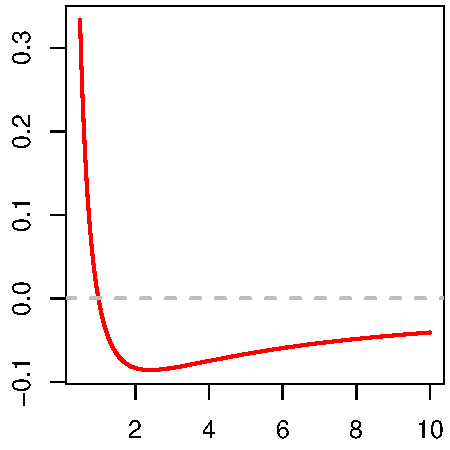
\includegraphics[width=\maxwidth]{figure/one_dimensional_loglik} 

\end{knitrout}
Which is be seen to have a unique root.
However, the log-likelihood $\ell$ is not log-concave since a differentiable function of one variable is concave if and only if its derivative is monotonically non-increasing.




\section{Negative semi-definite hessian in stationary points}
\label{sec:negativedefinite}
This section proves that the hessian is negative semi-definite in all stationary points.
The log-likelihood in \eqref{eq:loglik}, assuming $\nu$ fixed, obey
\begin{align}
  2\ell(\vPsi)
  = k\nu\log|\vPsi| - \sum_{a=1}^k (n_a + \nu)\log|\vPsi + \vS_a|
\label{eq:loglik2}
\end{align}
up to an addition of a constant. The matrix cookbook by \citet{Petersen2008} has been a useful reference here\footnote{See equation (41, p.\ 8) and (59, p.\ 9) and pages 14 and 52-53 in \url{http://www2.imm.dtu.dk/pubdb/views/publication_details.php?id=3274}}.



\subsection{1.\ order derivatives}
From the log-likelihood expression, we compute the 1.\ order derivative $\nabla_\vPsi 2\ell(\vPsi)$ which is the matrix-valued function where each entry is given by
\begin{align}
  %\left(\frac{\partial 2\ell}{\partial \vPsi}\right)_{ij}=
  \frac{\partial 2\ell}{\partial \Psi_{ij}}
  = k\nu\tr\!\left(\vE^{ij}\vPsi^{-1}\right)
    - \sum_{a = 1}^k (\nu + n_a)\tr\!\left(\vE^{ij}\left(\vPsi + \vS_a\right)^{-1}\right).
\label{eq:dloglik}
\end{align}
where $\vE^{ij}$ is a matrix with ones at entries $(i,j)$ and $(j,i)$ and zeros elsewhere.
This $\vE^{ij}$ is introduced as the derivative is not straight-forward because of the symmetric structure of $\vPsi$. Had $\vPsi$ been unstructured, then $\frac{\partial}{\partial \vPsi}\log|\vPsi| = \vPsi^{-1}$.
However, when $\vPsi$ is symmetric we have that $\frac{\partial}{\partial \Psi_{ij}}\log|\vPsi| = \tr(\vE^{ij}\vPsi^{-1})$ which is to say $\frac{\partial}{\partial \vPsi}\log|\vPsi| = 2\vPsi^{-1} -\vPsi^{-1} \circ \vI$ where $\circ$ denotes the Hadamard product \citep[eq.\ (43) and (141)]{Petersen2008}.

The first order derivative lives in a $\binom{p+1}{2}$-dimensional vector space indexed by $(i,j)$, $i\leq j$, with basis vectors $\vE^{ij}$.




\subsection{2.\ order derivatives}
We proceed with the second order derivative $\nabla^2_\vPsi 2\ell(\vPsi)$ with entries given by
\begin{align*}
  \frac{\partial^2 2\ell}{\partial \Psi_{kl} \partial \Psi_{ij}}
  &= - k\nu\tr\!\left( \vE^{ij}\vPsi^{-1} \vE^{kl}\vPsi^{-1} \right) \\
  & + \sum_{a = 1}^k (\nu + n_a)
    \tr\!\left(
      \vE^{ij}\left(\vPsi + \vS_a\right)^{-1}
      \vE^{kl}\left(\vPsi + \vS_a\right)^{-1}
    \right),
\end{align*}
obtained by differentiation of \eqref{eq:dloglik} combined with
$\frac{\partial}{\partial \Psi_{ij}} \vPsi^{-1} = - \vPsi^{-1}\vE^{ij}\vPsi^{-1}$
for symmetric matrices \citep[eq.\ (40)]{Petersen2008} and the linearity of the trace operator.

The second order derivative is a $\binom{p+1}{2} \times \binom{p+1}{2}$-dimensional matrix indexed by $(i,j)$ and $(k,l)$, $i \leq j$, $k \leq l$.




\subsection{Negative semi-definiteness in stationary points}
With the above expressions we now show that the hessian is negative semi-definite in all stationary points (or, extrema).
Let $\vY = \sum_{(i,j)} y_{ij}E_{ij}$ be a symmetric matrix in the vector space where $\vY \neq \vec{0}$. The analog to $\vec{y}^\top \vec{A}\vec{y} = y_i \sum_{ij} A_{ij} y_j \leq 0$ in our vector space then becomes
\begin{align*}
  \sum_{i\leq j, k\leq j}
    Y_{ij}
    \left(\nabla^2_\vPsi 2\ell(\vPsi)\right)_{(i,j),(k,l)}
    Y_{kl} \leq 0
\end{align*}
which amounts to showing that
\small
\begin{align}
- k\nu\tr\!\left( \vY\vPsi^{-1} \vY\vPsi^{-1} \right)
+ \sum_{a = 1}^k (\nu + n_a)
    \tr\!\left(
      \vY\left(\vPsi + \vS_a\right)^{-1}
      \vY\left(\vPsi + \vS_a\right)^{-1}
    \right) \leq 0.
  \label{eq:negativedefinte}
\end{align}
\normalsize
Now, the positive-definiteness of $\vPsi$, let
\begin{align*}
  \vY &:= \vPsi^{-\frac{1}{2}} \vY \vPsi^{-\frac{1}{2}} \text{ and } \\
  \vS_a &:= \vPsi^{-\frac{1}{2}} \vS_a  \vPsi^{-\frac{1}{2}}.
\end{align*}
we can assume that $\vPsi = \vI$. Hence, the likelihood equation \eqref{eq:loglik2} equated to zero, becomes
\begin{align*}
  k\nu\vI = \sum_a(n_a + \nu)(\vI + \vS_a)
\end{align*}
which implies (by multiplication by $\vY^2$)
\begin{align}
  k\nu\tr(\vY^2)
  &= \sum_a (n_a + \nu)\tr\!\left(\vY^2(\vI + \vS_a)\right) \notag\\
  &= \sum_a (n_a + \nu)\tr\!\left(\vY(\vI + \vS_a)\vY\right).
  \label{eq:loglikequation}
\end{align}
We substitute \eqref{eq:loglikequation} into \eqref{eq:negativedefinte} to get
\begin{align*}
  &\sum_a (n_a + \nu)\tr\left(\vY (\vI + \vS_a) \vY (\vI + \vS_a) - \vY (\vI + \vS_a) \vY \right) \\
  &=  \sum_a (n_a + \nu)\tr\!\Big( \vY (\vI + \vS_a) \vY \big[ (\vI + \vS_a)  - \vI \big]\Big)
  \leq 0
\end{align*}
Since $\vS_a$ is positive semi-definite, it can be diagonalized $\vS_a = \vU_a \vD_a \vU_a^\top$ by the spectral theorem where the diagonal matrix $\vD_a \succeq 0$ (all non-zero entries are positive) and $\vU_a$ is orthonormal (i.e.\ $\vU_a\vU_a^\top = \vU_a^\top\vU_a = \vI$). Using the diagonalization,
\begin{align}
  \sum_a (n_a + \nu)\tr\!\Big(
    \underbrace{\vU^\top \vY (\vI + \vS_a)^{-1} \vY \vU}
    \big[ (\vI + \vD_a)^{-1}  - \vI \big]
  \Big)
  \leq 0
  \label{eq:loglikequation2}
\end{align}
where the underbraced matrix is positive semi-definite and hence have non-negative diagonal elements.
Furthermore, since $\vD_a$ is diagonal also with non-negative elements, the diagonal matrix $(\vI + \vD_a)^{-1}  - \vI$ clearly have non-positive entries and is thus negative semi-definite.

Since the trace of a matrix product is the sum of the element-wise products, the trace (and thus the sum) will always be non-positive and hence \eqref{eq:loglikequation2} will always hold.

\section{log-likelihood of the precision}
\label{sec:precisionloglik}
Suppose we have $k$ i.i.d. realizations, $\vDelta_1, ..., \vDelta_k$, from the Wishart distribution given in equation \eqref{eq:precisiondensity}. The corresponding log-likelihood can be computed straight-forwardly:
\begin{align*}
  \ell(\vTheta | \vDelta_1, ..., \vDelta_k)
  &= \sum_{i = 1}^k \log f(\vDelta_i | \vTheta) \\
  &= \sum_{i = 1}^k \log
    \frac{|\vTheta|^{-\frac{\nu}{2}}}{
      2^{-\frac{vp}{2}}
      \Gamma_p\!\left(\frac{\nu}{2}\right)}
    |\vDelta_i|^\frac{\nu - p - 1}{2}e^{-\frac{1}{2}\tr(\vTheta^{-1}\vDelta_i)}\\
   &= c + \sum_{i = 1}^k
     -\frac{\nu}{2} \log |\vTheta|
     -\frac{1}{2}\tr(\vTheta^{-1}\vDelta_i) \\
   &= c + \frac{\nu k}{2}
     \left(
       \log |\vTheta| +
       \tr\!\left(\vTheta^{-1} \frac{1}{\nu k}\sum_{i = 1}^k\vDelta_i\right)
     \right).
\end{align*}
The last expression is to be maximized with respect to $\vTheta$ and can be recognized as the MLE problem in a multivariate Gaussian distribution. Hence,
\begin{align*}
  \vTheta = \frac{1}{k \nu} \sum_{i = 1}^k \vDelta_i,
\end{align*}
is the MLE in this model.


\section{Model and notation overview}
Let $\vDelta_i = \vSigma_i^{-1}$, $\vTheta = \vPsi^{-1}$, and $\vS_i = \vX_i^\top \vX_i$. Then the following equivalences hold.
\begin{equation*}
\begin{aligned}
  \vSigma_i &\sim \calW^{-1}_p(\vPsi, \nu) \\
  \vX_i | \vSigma_i &\sim \calN_p(\vec{0}_p, \vSigma_i) \\
  &\Updownarrow \\
  \vSigma_i | X_i  &\sim \calW^{-1}_p(\vPsi + \vS_i, \nu + n_i)
\end{aligned}
\begin{aligned}
\quad
&\Longleftrightarrow \\
&\Longleftrightarrow \\
\\
&\Longleftrightarrow
\quad
\end{aligned}
\begin{aligned}
  \vDelta_i &\sim \calW_p(\Theta, \nu) \\
  \vX_i | \vDelta_i &\sim \calN_p(\vec{0}_p, \vDelta_i^{-1}) \\
  &\Updownarrow \\
  \vDelta_i | X_i  &\sim \calW_p((\vTheta^{-1} + \vS_i)^{-1}, \nu + n_i)
\end{aligned}
\end{equation*}

\listoffixmes


\end{document}

